\documentclass[aps,prr,reprint]{revtex4-2}
\bibliographystyle{apsrev4-2}

\usepackage{graphicx}% Include figure files
\usepackage{svg}
\usepackage{dcolumn}% Align table columns on decimal point
\usepackage{bm}% bold math
\usepackage{braket}
\usepackage{amsmath}
\usepackage{amssymb}
\usepackage{hyperref}
\usepackage{url}
\usepackage[normalem]{ulem}

\hypersetup{hypertex=true,
colorlinks=true,
linkcolor=blue,
urlcolor = blue,
citecolor=blue}


\usepackage{color}
\newcommand{\mb}[1]{{\color{cyan}#1}}
\newcommand{\jw}[1]{{\color{red}#1}}
%\usepackage{hyperref}% add hypertext capabilities
%\usepackage[mathlines]{lineno}% Enable numbering of text and display math
%\linenumbers\relax % Commence numbering lines


\begin{document}

\title{Walsh-Floquet Theory of Periodic Kick Drives}

\author{James Walkling}
\email{jamwalk@pks.mpg.de}
\author{Marin Bukov}%
%\email{mgbukov@pks.mpg.de}
\affiliation{%
 Max Planck Institute for the Physics of Complex Systems, Nöthnitzer Strasse 38, 01187 Dresden, Germany
}%

%\date{\today}

\begin{abstract}
Periodic kick drives are ubiquitous in digital quantum control, computation, and simulation, and are instrumental in studies of chaos and thermalization for their efficient representation through discrete gates. However, in the commonly used Fourier basis, kick drives lead to poor convergence of physical quantities.
Instead, here we use the Walsh basis of periodic square-wave functions to describe the physics of periodic kick drives.  
In the strongly kicked regime, we find that it recovers Floquet dynamics of single- and many-body systems more accurately than the Fourier basis, due to the shape of the system's response in time. 
To understand this behavior, we derive an extended Sambe space formulation and an inverse-frequency expansion in the Walsh basis. 
We explain the enhanced performance within the framework of single-particle localization on the frequency lattice, where localization is correlated with small truncation errors.
We show that strong hybridization between states of the kicked system and Walsh modes gives rise to Walsh polaritons that can be studied on digital quantum simulators.  
Our work lays the foundations of Walsh-Floquet theory, which is naturally implementable on digital quantum devices and suited to Floquet state manipulation using discrete gates.
\end{abstract}


\maketitle

Quantum simulation is a pillar of quantum technology with numerous successes in the study of localization, thermalization, chaos, and topology. These simulations fall under two main categories: analogue and digital. For each of these categories, periodic driving is instrumental in the investigation of non-equilibrium physics within the paradigm of Floquet theory and the design of synthetic matter via ``Floquet engineering" \cite{Floquet1883, Bukov2015, Oka2019}. Analogue harmonic drives in optical lattices allow the simulation of gauge fields and topological models that are inaccessible in natural materials alongside dynamically induced localization \cite{Eckardt2017, BlochRev2017, AidelsburgerRev2018, SchaferRev2020}. On digital platforms, inherently non-equilibrium Floquet phases of matter can be simulated, such as discrete time crystals \cite{Sacha2017,Sondhi2019,Else2020, Yao2023,moon2024experimental}. Beside exactly implementing discrete stepwise-continuous protocols, arbitrary time dependence can be realized on digital platforms through Trotterization, which introduces an associated discretization (Trotter) error; it can cause Floquet heating in the system, and its mitigation or potential beneficial use is an active area of research \cite{Heyl2019, Wurtz2022, Kivlichan2020, Hongzheng2023}.

\begin{figure}[t!]
    \centering
    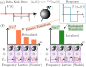
\includegraphics[scale=1]{../visual_elements/figs/loc_schematic.pdf}
    \caption{(a) A kicked system (represented as a spin-$1/2$) obeying the Schrödinger equation generically has a square wave response in the observables, via the micromotion $\ket{u_n(t)}$. (b) frequency lattice states in the tensor product of the physical spin Hilbert space, $\mathcal{H}$, and the space of periodic functions, $\mathcal{L}_\odot$ [schematic]. Depending on the choice of basis, the response is localized on the frequency lattice labeled by mode number, $m$. Wavefunctions are defined by $\braket{\uparrow |u_n(t)} = \sum \psi_f(m) f_m(t)$ where $f_m(t)$ represents Fourier or Walsh modes.
    }
    \label{fig:IntroFig}
\end{figure}

Periodic kick drives composed of delta function trains are exactly expressible on digital platforms. A paradigmatic example is the kicked Ising model, which is key in the simulation of exactly-solvable unitary dynamics \cite{Akila2016, Bertini2018, Bertini2019,Gopalakrishnan2019, AltmanRev2021, Ho2022}. Even beyond digital platforms, kick drives exhibit rich quantum dynamics; they give rise to non-ergodic and chaotic behavior~\cite{Haake1987, Chaudhury2009, Neill2016, Sieberer2019} and play a key role in large classes of quantum control protocols~\cite{Hahn1950,Tanner1968, Hans2020, Lasek2023}.

To solve perturbatively for the Floquet dynamics of such systems, a periodic basis with period $T=2\pi/\omega$ and frequency $\omega$ is used. In the frequency lattice construction \cite{Sambe1973,Eckardt2015}, the periodic part of the Floquet response -- the micromotion -- is expanded in the space of periodic functions $\mathcal{L}_\odot$, see~Fig.~\ref{fig:IntroFig}. The ``lattice" here refers to the labelling of Fourier basis functions $\exp(im\omega t)$ with $m \in \mathbb{Z}$. The frequency lattice is infinite; to study it numerically, the effective Hamiltonian matrix must be truncated, yielding basis-dependent results. For strongly periodically kicked systems, the commonly used Fourier series has notable disadvantages: a kick drive has constant Fourier series coefficients with no sensible cut-off; moreover, the cut-off process induces a strong ringing distortion called the ``Gibbs phenomenon" (see~Fig.~\ref{fig:Walsh}(c)) \cite{Hewitt1979}. While these effects can be mitigated, they point to the inadequacy of the Fourier basis to analyze digital drives. 



In this work, we introduce the periodic Walsh functions $\{W_m(t)\}$ as an alternative basis for $\mathcal{L}_\odot$. The Walsh basis is a set of periodic, orthonormal, piecewise-constant functions that only take values $\pm 1$ as shown in Fig.~\ref{fig:Walsh}(a). Historically, it was used extensively in signal processing and has also seen a recent revival in physics~\cite{Walsh1923, Fine1949, golubov2012, Hayes2011, Shukla2023, zylberman2024, Pagano2024, Votto2024}. The Walsh basis truncates via discretizing the signal in real space with a time step $T/N$ where $N$ is the number of basis functions. Dynamical equations contain the time derivative; when treated explicitly as the time translation generator, we show that it takes a block diagonal form in the Walsh basis with an identical spectrum to the Fourier.

Under strong digital driving, quantum systems have a piecewise continuous response. We demonstrate that for a system driven with a delta function train, the response can be captured by far fewer non-zero coefficients in the Walsh basis as compared to the Fourier basis. Directly tied to this, we find that the error in the quasienergies can be orders of magnitude smaller in the Walsh than the Fourier basis when truncating to the same number of modes. To illustrate this, we calculate the time evolution of periodically-kicked single-particle and many-body mixed-field Ising model (MFIM).


We interpret the improved performance in the Walsh basis via a single-particle localization problem; for an accurate description of the dynamics under truncation of the frequency lattice, we find that the response must be localized in the frequency lattice to minimize the truncation error. We quantify localization through the participation entropy and demonstrate that strong localization on the frequency lattice corresponds to a more accurate description of the dynamics via the error in the quasienergies. 

Our work demonstrates that the Walsh basis can offer a marked advantage over the Fourier basis in the setting of strongly kicked systems. This has applications for digital quantum simulators where many toy models for chaos and thermalization use kick drives.

\textit{Walsh Basis in a Nutshell---}%
The Walsh basis $\{W_m(t)\}$ is a set of $N=2^n$ orthonormal step functions on $[0,T]$. For $n=1$, the Walsh basis elements are just the rows of the Hadamard matrix, 
\begin{equation}
\mathbb{H}_2 = \begin{bmatrix}
    1 & 1 \\
    1 & -1 \\
\end{bmatrix}.
\label{eqn:HadamardMatrix}
\end{equation}
To find the Walsh functions for larger $n$, one uses the Hadamard matrix of order $2n$ which is formed by taking the tensor product $n$ times of $\mathbb{H}_2$. An example of the corresponding matrix for $n=2$ is shown in Fig.~\ref{fig:Walsh}(b). These periodic functions are defined by a set of points $t_j = j T/2^n$ where $j=0,1,\cdots, 2^n-1$. Away from these points, the values of the Walsh functions come from interpolating in a piecewise constant manner (see Fig.~\ref{fig:Walsh}(a)). 
We label the states according to natural ordering \cite{Zhihua1983}; this means that the same function will change its label in the basis, for different $N$. For instance, we can label the Walsh function with a single root (e.g., $W_2(t)$ in Fig.~\ref{fig:Walsh}(a)) as $W_{N/2}(t)$, since this gives the correct label for any $N$. 
In Fig.~\ref{fig:Walsh}(a) and (b), we illustrate the Walsh functions on the real line and the character table from which they are derived for $n=2$. 

\begin{figure}[t]
    \centering
    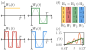
\includegraphics[scale=1]{../visual_elements/figs/walsh_examples.pdf}
    \caption{
    (a) Walsh basis functions for $N=4$ basis elements along with related trigonometric functions in a dashed line. This correspondence only works for $N=4$ since the roots of the Walsh functions are not evenly spaced for $N > 4$. 
    (b) construction of the Walsh basis from the Hadamard matrix for $N=4$. 
    (c) example of representing a function with discontinuities in different bases. The Walsh (green) consistently undershoots for smooth variation; by contrast, the Fourier  (orange) oscillates wildly near sharp discontinuities (Gibbs phenomenon) for a periodic sawtooth wave (dashed black).}
    \label{fig:Walsh}
\end{figure}



Both the Walsh and Fourier are complete bases such that their representations of functions should be equivalent; however, under truncation, the corresponding approximations differ. To render the frequency space finite, the Fourier basis applies a sharp cutoff which discards any coefficients associated with higher frequencies. By contrast, the Walsh basis maps different frequencies onto each other; the time discretization in the Walsh basis leads to distortion of the signal (aliasing) because it cannot resolve the shorter lengthscale features of a function \cite{Nyquist1928}. If higher frequencies carry significant weight, as in the presence of singularities, discarding higher frequencies in the Fourier basis suggests that the Walsh basis can outperform. Further details of the construction of the Walsh basis, and the difference in the Walsh and Fourier coefficients due to the aliasing effect are discussed in detail in the Supplementary Material. We now detail the use of the Walsh basis to solve the Floquet problem. 



\textit{Quasienergy operator in the Walsh basis---}%
The solution to the Floquet problem, the evolution of a periodically driven system with Hamiltonian $\hat{H}(t) = \hat{H}(t+T)$, is given by the eigenstates and eigenvalues of the Floquet Hamiltonian, $H_F$, alongside the kick operator, $K(t)$, cf.~Supplementary Material. 

The eigenstates and eigenvalues of the Floquet Hamiltonian can be found from the quasienergy operator,
\begin{equation}
    \hat{Q}(t) = \hat{H}(t) - i\partial_t.
    \label{eqn:Qmatrix}
\end{equation}
To diagonalize it, we write it as $\bar{Q}$ in an extended frequency space (Sambe space \cite{Sambe1973}), $\mathcal{F}= \mathcal{H} \otimes \mathcal{L}_\odot$. $\mathcal{H}$ is the physical Hilbert space associated with $\hat{H}(t)$, and we promote the periodic time-dependence to its own Hilbert-space, $\mathcal{L}_\odot$ \cite{Eckardt2015}. The inner product on $\mathcal{F}$, is $\langle \langle u | v \rangle \rangle = T^{-1}\int_0^T \text{d} t \braket{v(t)|u(t)}$. 


The operator $\bar{Q}$ has eigenvalues $\varepsilon_{nm} = \varepsilon_n + m\omega$, where $m \in \mathbb{Z}$. These eigenvalues, known as quasienergies, are defined modulo $m\omega$. In figures, we rescale to define dimensionless Floquet phases $\theta_n=\varepsilon_n T$. The corresponding eigenvectors, the Floquet modes, are expressed as $\ket{u_{nm}(t)} = e^{im\omega t} \ket{u_n(t)}$, with the phase factor accounting for the modularity. The integer $m$ is referred to as a photon index, since it can be intuitively thought of as the number of photons dressing the state. Previously, the Fourier basis has been used to decompose $\ket{u(t)}$ as $\ket{\alpha m(t)}= \ket{\alpha}e^{im\omega t}$, and these are expressed as $\ket{\alpha,m}\rangle$ in the extended space.

To instead write the operator $\bar{Q}$ in the Walsh basis, one needs to handle the derivative operator with care; on a piecewise-constant basis, the derivative is not necessarily equal to the generator of continuous time translations as it is for a continuous basis. Indeed, in the Walsh basis, the derivative is not the generator of translations for finite $N$, as becomes evident from their different spectra. However, the translation generator, $\hat{G}$, defined thoroughly in the Supplementary Material, agrees exactly with the truncated spectrum of the derivative for any $N$. Hence, in the Walsh basis, $\hat{G}$ is used in place of the derivative in Eq.~\eqref{eqn:Qmatrix}; in the extended space associated with the Walsh basis, Eq.~\ref{eqn:Qmatrix} reads as $\bar{Q}=H-i\hat{G}$. Properties of $\hat{G}$ in the Walsh basis, such as its block-diagonality, and truncation of the frequency lattice are discussed further in the Supplementary Material.

\begin{figure}[t!]
    \centering
    \includegraphics[scale=1]{../visual_elements/figs/spin_kick.pdf}
    \caption{Single-particle quasienergies from a kick drive, see Fig.~\ref{fig:IntroFig}(a). 
    (a) is the quasienergy spectrum for $\omega =10$ and $h_z=4.5$ showing the superior performance of the Walsh basis over the Fourier. 
    (b) quantifies the error over a range of parameters, showing that Walsh outperforms Fourier the most for strong kick drives. In the orange region, the Fourier basis better approximates the quasienergies, and in the green region the Walsh performs better. $N=32(31)$ modes used in both plots.
    }
    \label{fig:SPerror}
\end{figure}

\begin{figure}[t]
    \centering
    \includegraphics[scale=0.99]{../visual_elements/figs/mb_spin_kick.pdf}
    \caption{(a) Many-body quasienergy spectrum for $L=3$ spins and $N{=}32(31)$ modes with $J=1$ and $h_zT=1.1\pi$. The Walsh basis outperforms the Fourier. (b) Comparison of the error in the dimensionless quasienergy phases calculated using the Walsh and Fourier basis to the same level of truncation, $N{=}64(63)$ modes, for $L=6$ spins. Green indicates that Walsh is more accurate than the Fourier, and orange means the opposite.
    Apart from very small kick fields, the Walsh basis outperforms over a large parameter regime. At large kick fields, in the black region, there is an error w.r.t.~the exact solution by more than 1\% in both bases.
    }
    \label{fig:MBerror}
\end{figure}

\textit{Bases comparison for a kicked Ising model---}%
We focus on a kick drive which is an up-down kick with zero average, $V(t)$, as illustrated in red in Fig.~\ref{fig:IntroFig}(a); this choice is motivated by its anti-derivative being a single Walsh mode, and is made for simplicity. The $\bar{Q}$ operator for the Fourier and Walsh bases is shown in the Supplementary Material for the case of this kick drive.

To compare the bases, we quantify their accuracy in reproducing the Floquet dynamics via the quasienergy phases $\theta_n$ for the MFIM:
\begin{equation}
    H = - \sum_{i=0}^{L-2} J \sigma_i^z \sigma_{i+1}^z 
    - \sum_{i=0}^{L-1} \big( h_z \sigma_i^z + h_x V(t) \sigma_i^x \big).
    \label{eqn:MFIM}
\end{equation}
The error is defined by subtracting off the exact result: $\Delta \theta_\text{basis}=|\theta_{\text{basis}}-\theta_{\text{exact}}|$.
When comparing the Walsh with the Fourier basis Walsh always has an even number of modes (i.e., $N=32$), whereas the Fourier basis benefits from having an odd number due to symmetry (i.e., $N=31$).

First comparing the two in the single-particle limit of Eq.~\eqref{eqn:MFIM} ($J=0$ and $L=1$), we plot the quasienergy spectrum and errors at finite truncation in Fig.~\ref{fig:SPerror}(a) and (b) respectively. Although the Fourier basis outperforms the Walsh basis for weakly kicked drives, the Walsh performs much better than the Fourier basis for strongly kicked drives. For zero field strength, the response of the spin, $\ket{u(t)}$, is time-independent, and this is a single mode in both bases; hence, they perform equally well. For weak kicking, the smooth response is marginally better captured by the Fourier (Fig.~\ref{fig:SPerror}(a) for small kick field shows very little difference). When $h_z \sim \pi/4$, the discontinuities are significant enough to favor the Walsh basis. Along the line $h_z=0$, the exact quasienergies are zero which is perfectly calculated by Fourier due to its reflection symmetry for an odd number of modes.



In the many-body case (Fig.~\ref{fig:MBerror}(a)), we see that the Walsh basis (green) is orders of magnitude closer to the exact numerics than the Fourier (orange) for intermediate kick strengths less than $\pi/2$. In addition, the Walsh basis (green) outperforms the Fourier basis (orange) over a broad parameter range as illustrated in Fig.~\ref{fig:MBerror}(b). For larger values of the kick field, $h_x$~\footnote{$h_x$ is a dimensionless quantity in natural units since it is the amplitude of a delta function drive. $h_z$ is dimensionful since it just multiplies some time independent term.}, the Walsh basis outperforms by at least an order of magnitude. These larger $h_x$ are relevant to several models involving kick drives to explore thermalization, localization and non-equilibrium phases since this is where the drive plays a significant role. Alongside the qualitative reasons we discussed for the poor behavior of the Fourier basis in the presence of kick drives, we now give compelling reasons why the Walsh is the appropriate basis.

\textit{Understanding errors via Frequency lattice localization---}%
There are several intuitive explanations for why the Walsh basis outperforms the continuous Fourier basis for kick drives. Since kick drives are periodic in frequency space with constant Fourier coefficients $c_n \sim \mathcal{O}(1)$, imposing a cutoff is a poor approximation since we discard infinitely many relevant frequencies. The aliasing effect creates several copies of the true spectrum (see Supplementary Material), which preserves the translational symmetry of the kick drive in frequency space, giving the Walsh basis an advantage in representing these singular functions at finite truncation. 

Physically, accurate reproduction of the dynamics under truncation can be understood through localization on the frequency lattice, $\mathcal{L}_\odot$. The response of the system to the drive, encoded by the Floquet states $\ket{u_n(t)}$, can have many modes when expanded in a given time-periodic basis. Through truncation, we implement a cutoff on these modes. Hence, if $\ket{u_n(t)}$ are well-localized in photon space for a given basis, we expect to get a good approximation by truncating in that basis. We emphasize that the basis should be optimized to the response, $\ket{u_n(t)}$, rather than the drive. Rather surprisingly, this means that the Walsh basis is a poor basis to capture dynamics induced by square wave drives despite having a single mode spectrum (see Supplementary Material).

\begin{figure}[t!]
    \centering
    \includegraphics[width=\linewidth]{../visual_elements/figs/loc_vs_error.pdf}
    \caption{(a) Spin-up component of the response of a kicked two-level system system, defined via $\braket{\uparrow| u(t)} = \sum_m \tilde{u}_m f_m(t)$, where $f_m(t)$ denotes the orthonormal basis (Fourier, Walsh), see legend. Main plot shows the modes; the inset -- their time evolution, which is close to a square wave at high frequencies. Dashed (solid) lines indicate the low- (high-) frequency regime. At high frequency, the signal is strongly localized in the Walsh basis, and follows a $1/m$ power law decay otherwise. (b) difference in quasienergy errors, $\langle \Delta \theta \rangle \equiv\Delta \theta_{FW}=|\Delta \theta_F|- |\Delta \theta_W|$, and photon participation entropy ($\Delta S$ Eq.~\eqref{eqn:PPE}) highlighting the similarity between localization and associated error, scaled by a factor of $10^2$ (see text box). The errors are computed over all spins; localization is only shown for the spin-up component. The singular behavior near $h_zT=0$ comes from the degeneracy of $U(T,h_z=0)=\mathbf{1}.$
    Data obtained using Eq.~\eqref{eqn:MFIM} with $L=1$; for (a) $\omega, h_x= 10, \pi/2$.}
    \label{fig:localization}
\end{figure}

In the Fourier case, the localization problem is a general Wannier-Stark model in 1D; there is a linearly varying on-site potential (due to $-i\partial_t \equiv -i \hat{G}$) along with some tunneling elements that appear off-diagonal corresponding to an effective Hamiltonian in Sambe space $\bar{H}= \sum_j j \omega \mathbb{I} \otimes \hat{a}^\dagger_j \hat{a}_{j} + \sum_{j,j'} \hat{H}_{j-j'} \otimes \hat{a}^\dagger_j \hat{a}_{j'},$ where the operator $\hat{a}^\dagger_j$ creates a virtual ``photon" with frequency $j\omega$ on the space $\mathcal{L}_\odot$. 

The case of a harmonic drive is well-approximated by the Fourier basis; this corresponds to nearest neighbor tunnelling and exponentially localized eigenstates. By contrast, a generic kick drive has eigenstates that do not appear to decay with distance at all in the Fourier basis due to the all-to-all coupling in $\bar{H}$ with constant magnitude. 

For the Walsh basis, the non-diagonal form of the derivative means that the mapping to a Wannier-Stark ladder is no longer possible. However, in the high-frequency regime, it is possible to approximate the time-dependence of the response, $\ket{u_n(t)}= \exp(- i K(t)) \ket{u_n(0)}$, using the van Vleck expansion \cite{Bukov2015,Goldman2014}. The time evolution of the response is generated by the kick operator $K(t)$,
\begin{align}
    \exp(-i K(t)) = \exp \bigg[ -i\int^t \text{d}s \, H(s) \bigg] + \mathcal{O}(\omega^{-2}).
    \label{eqn:kickop}
\end{align}
% The operator $K(t)$ generates the time evolution of the Floquet modes:
% \begin{equation}
%     \ket{u_n(t)} = \exp(- i K(t)) \ket{u_n(0)}.
% \end{equation}
Hence, in the high-frequency regime, using Eq.~\eqref{eqn:kickop}, we can guess at the form of the time-evolution and pick a basis accordingly. In particular, the Walsh basis performs well for the kick drive $V(t) =\dot{W}_{N/2}(t)$ since the response, $e^{-iK(t)} {\propto} W_{N/2}(t) + \mathcal{O}(\omega^{-2})$ (inset of Fig.~\ref{fig:localization}(a)). 
Away from the high-frequency regime, we can turn to other indicators of localization. 

We can view frequency lattice localization as a semi-quantitative predictor for the error in the quasienergies. 
The errors can be quantified via the localization of the modes, $\ket{u_n(t)}$, using the photon participation entropy,
\begin{equation}
    S= -\sum_{m} P_m \ln(P_m),
    \label{eqn:PPE}
\end{equation} 
where we trace over states $\ket{\alpha}\in\mathcal{H}$ to define a probability of occupying the $m$th mode, $P_m=\sum_\alpha|\langle \braket{\alpha m|\alpha m}\rangle|^2$, independent of the physical state $\ket{\alpha}$. While other localization measures such as the inverse participation ration (IPR) also capture this localization, the logarithm present in the photon participation entropy makes it drop off in value less steeply for extended states and leads to a marginally better comparison with the error.
In Fig.~\ref{fig:localization}(b) and (c), we see that a large photon participation entropy (delocalized in the up spin component) corresponds to a larger error. The participation entropy qualitatively predicts when solutions from truncation are more accurate. This demonstrates clearly how choosing the optimal basis of $\mathcal{L}_\odot$ for a given drive can be understood as a problem in single-particle localization physics. We have omitted the spin-down component since this suffers from resonance effects in the first Floquet Brillouin zone. 

Resonances in the spectrum can lead to disagreement between error and delocalization due to strong hybridization between physical and photonic degrees of freedom, a.k.a.~polariton states; averaging over the physical degrees of freedom becomes a coarse approximation. Depending on parameters, the polaritons behave differently. Arbitrarily weak drive generically gives a ``Fourier" polariton where one spin component hybridizes with $\exp(i m\omega t)$. However, for kick field $h_x=\pi/2$ and $h_z T\ll1$, one observes a ``Walsh" polariton where a component hybridizes with $W_m(t)$.

Both the spin-down component and polariton are discussed further in the Supplementary Material. 

\textit{Discussion and Outlook---}%
We have shown that Floquet analysis can be performed consistently in the Walsh basis. For kicked drives, we demonstrated that the Walsh basis more accurately describes the time evolution, when compared to Fourier, at a given truncation level in both single- and many-particle systems. The superior performance of the Walsh basis can be traced back to the response of the system (rather than the drive): the square-wave time-dependence of the Floquet modes is naturally expressed in the Walsh basis. Physically, we explain the increase in truncation error as a delocalization of the Floquet modes on the frequency lattice ($\mathcal{L}_\odot$); measures of localization, such as the photon participation entropy, capture the relative accuracy of periodic bases in describing the Floquet dynamics. 

While localization entropy generally predicts the error well, it can jump sharply near resonances. In the high-frequency regime, resonances introduce factors $e^{im\omega t}$ into the response, delocalizing it across several modes in non-Fourier bases, even if it remains confined within a particular Floquet zone. When states of $\mathcal{H}$ in a Floquet zone have different localization behavior, tracing over $\mathcal{H}$ can lead to an incorrect error estimate. Moreover, convergence is not generally guaranteed in the Fourier or the Walsh basis, as the number of modes $N\to\infty$. However, there is still asymptotic validity in the solutions obtained for finite $N$.

In practice, the Walsh basis has recently seen a surge of interest in several research areas of quantum physics. 
It is being actively investigated for the advantages it offers over alternative bases in both theoretical and experimental settings in quantum sensing and control~\cite{Wang2024, Pagano2024}. The Walsh basis offers a promising tool for designing digital shortcuts-to-adiabaticity on quantum simulators, such as by extending Floquet counterdiabatic driving~\cite{Schindler2024,schindler2024geometric, xichen2024, Sun2022, Wurtz2022} to periodically kicked drives.
Similarly, in quantum computation and simulation, recent works have investigated the Walsh basis to efficiently encode the action of Pauli gates~\cite{Votto2024, Georges2025, zylberman2024}. Our study gives rise to a natural reformulation of the inverse-frequency expansion, which reduces the computational cost of effective Hamiltonian calculations by eliminating contributions from certain expansion orders (see Supplementary Material). 
Curiously, interaction with the drive can also give rise to Walsh polaritons (Fig.~S1 (d)) in the presence of particularly strong kicks -- where spin or particle degrees of freedom hybridize with the drive in one of the Walsh modes; this opens up exciting and natural new possibilities for studying polariton physics on digital quantum simulators.

Advancing the toolbox of periodic drives, we have quantified the performance of the Walsh basis and established it as a competitive new tool. Our work opens up new pathways to think about and utilize digital Floquet drives on NISQ devices.



\begin{acknowledgments}
We thank A.~Eckardt, M.~Heyl, and R.~Moessner for fruitful discussions. 
Funded by the European Union (ERC, QuSimCtrl, 101113633). Views and opinions expressed are however those of the authors only and do not necessarily reflect those of the European Union or the European Research Council Executive Agency. Neither the European Union nor the granting authority can be held responsible for them.
Numerical simulations were performed on the MPIPKS HPC cluster.
\end{acknowledgments}


%\clearpage


\bibdata{bibliography}
\bibliography{bibliography}

\end{document}

